\documentclass[../main.tex]{subfiles}

\graphicspath{{../images/}}
\usepackage{ytableau}
\begin{document}

\section{Lecture (1/17/24)}
\barh 

\paragraph{Four Fundamental Forces}

\begin{itemize}
    \item Strong (gluon)
    \item Weak (W, Z)
    \item Electromagnetic (photon)
    \item Gravity (graviton?)
\end{itemize}

The `Standard Model' describe the first three forces and unifies the Strong and Weak Forces known as
the `Electroweak' force. So, the Standard Model does not include gravity.

\paragraph{The Standard Model (SM)}
\begin{itemize}
    \item Basic building blocks: spin 1/2 particles (fermions)

    \item Interaction between then are mediated by force carriers:
    spin 1 particles (vector bosons)
    
    \item How particles get mass? $\rightarrow$ Higgs Boson (spin 0)
\end{itemize}

The Range of Forces:
\begin{itemize}
    \item Strong: $10^{-15}$ m
    \item Weak: $10^{-18}$ ~ $10^{-16}$ m
    \item EM: $1/r^2$
    \item Gravity: $1/r^2$
\end{itemize}

The ranges of forces are related by
\begin{align*}
    R ~ \frac{e^{-r/a}}{r^2}
\end{align*}
where $a \approx 10^{-15}$ m for the Strong and Weak forces.

\paragraph{The Rise of Quantum Field Theory (QFT)}

Relativity + Quantum Mechanics $\rightarrow$ QFT

% 3 x 3 table
\begin{center}
    \begin{tabular}{c|c|c}
        & Macroscopic & Micro \\
        \hline
        SLOW & CM & Quantum Mechanics \\
        \hline
        FAST & Special Relativity & QFT \\
    \end{tabular}
\end{center}

\paragraph{QFT Discoveries}
\begin{itemize}
    \item Existence of anti-particles
    \item Spin-statistics theorem
    \item CPT Theorem (Charge conjugation, Parity, Time reversal)
\end{itemize}

\subsection*{Units!}
\begin{itemize}
    \item Mass: (kg) $\rightarrow$ (eV) from $E = mc^2$
\begin{align*}
    m_e &= \qty{0.5e6}{\electronvolt/c^2} \quad E_n = \frac{\qty{-13.6}{\electronvolt}}{n^2} \\
    m_p &= \qty{1}{\giga\electronvolt/c^2} \quad \qty{1}{\electronvolt} = \qty{1.6e-19}{\joule}
\end{align*}
    \item Momentum: $\frac{eV}{C} \rightarrow p = \frac{E}{c}$
    \item Energy: eV
\end{itemize}

\paragraph{Matter Fermions} are divided into two groups:
\begin{itemize}
    \item Leptons (electrons, muon, tau, neutrinos): Doesn't have the strong force
    \item Quarks (up, down, charm, strange, top, bottom): Feels the strong force 
\end{itemize}
e.g. the proton is made of 2 up quarks and 1 down quark (uud) and the Neurtron is (udd).

\paragraph{Quarks} make up composite subparticles (Hadrons) are held together by the strong force.
\begin{itemize}
    \item Mesons: 1 quark + 1 anti-quark $(q\bar q)$ e.g. pion, kaon...
    \item Baryons: 3 quarks $(qqq)$ e.g proton, neutron
\end{itemize}

Quark charges:
\begin{itemize}
    \item $Q = +2/3$ (up, charm, top)
    \item $Q = -1/3$ (down, strange, bottom)
\end{itemize}

\paragraph{Leptons} are fundamental particles
\begin{itemize}
    \item Charged electrically (-1)
    \begin{itemize}
        \item electron $(\qty{0.5}{\mega\electronvolt})$
        \item muon $(\qty{105}{\mega\electronvolt})$
        \item tau $(\qty{1.8}{\giga\electronvolt})$
    \end{itemize}
    \item Neutral (neutrinos)
    \begin{itemize}
        \item electron neutrino $\nu_e$
        \item mueon neutrino $\nu_\mu$
        \item tau neutrino $\nu_\tau$
    \end{itemize}
\end{itemize}

\paragraph{Crossing Symmetry}
\begin{align*}
    A + B &\rightarrow C + D \quad \textrm{Scattering} \\
    A &\rightarrow B + C + D \quad \textrm{Decay} \\
    A + \bar C &\rightarrow \bar B + D
\end{align*}
e.g. Neutron Decay
\begin{align*}
    n &\rightarrow p + e^- + \bar \nu_e 
\end{align*}
Sum rules to think about:
\begin{itemize}
    \item Baryon Number Conservation
    \item Lepton Number Conservation
    \item Electric Charge Conservation
\end{itemize}
another example:
\begin{align*}
    n + e^+ &\rightarrow p + \bar \nu_e \\
    p + e^- &\rightarrow n + \nu_e
\end{align*}

\href{https://phys.libretexts.org/Bookshelves/University_Physics/University_Physics_(OpenStax)/University_Physics_III_-_Optics_and_Modern_Physics_(OpenStax)/11%3A_Particle_Physics_and_Cosmology/11.03%3A_Particle_Conservation_Laws}{Particle Conservation Laws}

\newpage
\subsection*{Lecture 2: \hfill  1/22/24}
\hrule \vspace{10px}
\section{Relativistic Kinematics}
\hrule \vspace{10px}

\paragraph{Quiz 2 Review}

\begin{enumerate}
    \item The Baryon, Lepton, and Electric Charge are conserved in the Standard Model. 
    \item The Baryon and Lepton number ensure the stability of the proton.
    \item In Neutron Decay $n \rightarrow p + e^- + \bar \nu_e$, the weak force is responsible for
    the decay.
% 5x3 table
\begin{center}
    \begin{tabular}{c|c|c|c|c}
        & Strong & EM & Weak & Gravity \\
        \hline
        Strength & 1 & $10^{-2}$ & $10^{-7}$ & $10^{-40}$ \\
        \hline
        Time scale & $10^{-23}$ sec & $10^{-16}$ & $10^{-10}$ & $>$ yr\\
    \end{tabular}
\end{center}
    The decay rate is proportional to the coupling strength of the force $\Gamma \propto \alpha^2$.
    For the time scale is $\tau$ it is inversely proportional:
    \begin{align*}
        \tau \propto \frac{1}{\Gamma}
    \end{align*}
    \item The strong force is responsible for holding the nucleus together.
    \item 
\end{enumerate}

\paragraph{Experimental Discoveries}

To discover and observe particles, there are typically three ways:
\begin{enumerate}
    \item Scattering (cross section) 
    \item Decay (decay rate or lifetime)
    \item Bound states (binding energy/mass)
\end{enumerate}

\paragraph{Relativistic Kinematics} 4-vectors
\begin{align*}
    x^\mu = (ct, x, y, z) \quad \textrm{space-time} \\
    p^\mu = (E/c, p_x, p_y, p_z) \quad \textrm{momentum}
\end{align*}
where $x^\mu$ and $p^\mu$ are the space-time (position) four-vector and energy-momentum four-vector.

\subparagraph*{NOTE:} Totak four-momentum is conserved in all interactions.

Starting with the lorentz invariant
\begin{align*}
    p^\mu p_\mu = p^2
\end{align*}
using the Einstein-summation convention
\begin{align*}
    p^\mu p_\mu = \sum_{\mu = 0}^3 p^\mu p_\mu = p^2
\end{align*}
and the metric tensor
\begin{align*}
    g^{\mu\nu} = \begin{pmatrix}
        1 & 0 & 0 & 0 \\
        0 & -1 & 0 & 0 \\
        0 & 0 & -1 & 0 \\
        0 & 0 & 0 & -1 \\
    \end{pmatrix}
\end{align*}
we can write the lower momentum vector as
\begin{align*}
    p_\mu = p^\nu g_{\mu\nu} 
\end{align*}
thus
\begin{align*}
    p^\mu p_\mu &= p^\mu p^\nu g_{\mu\nu} \\
    &= \qt(\frac{E}{c})^2 + \vb{p} \cdot \vb{p} (-1) \\
    &= \qt(\frac{E}{c})^2 - \abs{\vb{p}}^2 \\
    &= m^2 c^2
\end{align*}
Using
\begin{align}
    E = \sqrt{\abs{\vb{p}}^2 + m^2 c^4}
\end{align}

\paragraph{Lorentz Transformation} At rest $\vb{p} = 0$ and $E = mc^2$.

In the Galilean transformation in the $x$ direction:
\begin{align*}
    x' &= x - vt \\
    y' = y \\
    z' = z \\
    t' = t
\end{align*}
where we assume absolute time, but in the Lorentz transformation:
\begin{align*}
    x' &= \gamma(\beta ct + x) \quad \beta = \frac{v}{c} \\
    ct' &= \gamma(t - \beta x) \quad \gamma = \frac{1}{\sqrt{1 - \beta^2}} \\
    y' &= y \\
    z' &= z
\end{align*}
In matrix form:
\begin{align*}
    \Lambda = 
    \begin{pmatrix}
        ct' \\
        x' \\
        y' \\
        z' \\
    \end{pmatrix}
    &= \begin{pmatrix}
        \gamma & -\beta\gamma & 0 & 0 \\
        -\beta\gamma & \gamma & 0 & 0 \\
        0 & 0 & 1 & 0 \\
        0 & 0 & 0 & 1 \\
    \end{pmatrix}
    \begin{pmatrix}
        ct \\
        x \\
        y \\
        z \\
    \end{pmatrix}
\end{align*}
and thus $p^\mu p_\mu$ is invariant under Lorentz transformation.

\paragraph{Massless particle:} From the energy momentum relation
\begin{align*}
    E^2 = \abs{\vb{p}}^2 c^2 + m^2 c^4
\end{align*}
The massless particle has energy $E = \abs{\vb{p}}c$. But we have to include the frequency (Planck)
relation from quantum mechanics as well:
\begin{align*}
    E = h \nu = \hbar \omega
\end{align*}
And in the SM photons and neutrinos are massless thus
\begin{align*}
    p^2 = p^\mu p_\mu = m^2 c^2 = 0
\end{align*}

\paragraph{Collisions} Non-relativistic vs. Relativistic

Non-relativistic:
\begin{itemize}
    \item Elastic (KE conserved)
    \item Inelastic (KE not conserved)
\end{itemize}
Relativistic:
\begin{itemize}
    \item Elastic (KE conserved) e.g. particle splitting into two
    \item Inelastic (KE not conserved) or Rest energy and mass e.g. colliding two particles to form
    a new particle
    \begin{itemize}
        \item KE increases (Explosive)
        \item KE decreases (Sticky)
    \end{itemize}
\end{itemize}
In the extreme case:
\begin{align*}
    A &+ B \rightarrow C \quad \textrm{inverse decay} \\
    A &\rightarrow B + C \quad \textrm{decay}
\end{align*}

\paragraph{Example} $\pi^+ \rightarrow \mu^+ + \nu_\mu$ (decay)

The Rest energies are $m_{\pi^+} = \qty{135}{\mega\electronvolt/c^2}$,
$m_{\mu^+} = \qty{105}{\mega\electronvolt/c^2}$, and $m_{\nu_\mu} = 0$. But this energy is lost
through the kinetic energy of the muon and muon-neutrino.

The momentum before is just the momentum of the pion
\begin{align*}
    p_i = p_{\pi} = 0
\end{align*}
since it is startionary. Afterward the momentum is split between the muon and neutrino
\begin{align*}
    p_f = p_{\mu} + p_{\nu_\mu}
\end{align*}
where energy and momentum is conserved:
\begin{align*}
    \vb{p}_\mu &= -\vb{p}_{\nu} \\
    m_{\pi} c^2 &= E_{\mu} + E_{\nu_\mu} 
\end{align*}

\paragraph{4-momentum conservation}
\begin{align*}
    p_{before} &= p_{after} \\
    p_{\pi} &= p_{\mu} + p_{\nu_\mu}
\end{align*}
since the massless particle has no momentum from the energy momentum relation
\begin{align*}
    p_\nu &= p_\pi - p_\mu \\
    p_\nu^2 &= (p_\pi - p_\mu)^2 \\
    &= p_\pi^2 - 2p_\pi p_\mu + p_\mu^2 \\
    0 &= m_\pi^2 c^2 + m_\mu^2 c^2 - 2\frac{m_\pi c^2}{c} \frac{E_\mu}{c} \\
    2E_\mu m_\pi &= (m_\pi^2 + m_\mu^2) c^2 \\
    E_\mu &= \frac{m_\pi^2 + m_\mu^2 - m_\nu^2}{2m_\pi} c^2 \\
\end{align*}

Another way is finding
\begin{align*}
    p_\pi = p_\mu + p_\nu
\end{align*}
rewritten as
\begin{align*}
    p_\mu = p_\pi - p_\nu
\end{align*}
squaring both sides gives
\begin{align*}
    p_\mu^2 = p_\pi^2 - 2p_\pi p_\nu + p_\nu^2
\end{align*}
and since $p_\nu^2 = 0$ we have
\begin{align*}
    p_\mu^2 = p_\pi^2 - 2p_\pi p_\nu
\end{align*}
which implies
\begin{align*}
    m_\mu^2 c^2 = m_\pi^2 c^2 - 2m_\pi E_\nu
\end{align*}
the Planck relation tells us
\begin{align*}
    E_\nu = \abs{\vb{p}_\nu} c = \abs{\vb{p}_\mu} c
\end{align*}
thus
\begin{align*}
    2 m_\pi \abs{\vb{p}_\mu} c = (m_\pi^2 - m_\mu^2) c^2
\end{align*}
and
\begin{align*}
    \abs{\vb{p}_\mu} = \frac{m_\pi^2 - m_\mu^2}{2m_\pi} c
\end{align*}

\paragraph{Scattering experiments}

\begin{itemize}
    \item Head-on collision: (LHC)
    \item Fixed target collision: Beam of protons hitting a target (e.g. Carbon) (SLAC)
\end{itemize}  
From momentum conservation, the head-on collision is more energy efficient as it loses the minimum
amount of energy. The created particle is at rest, thus the energy is the rest energy. But the Fixed
target collision has a higher energy loss since the particle loses energy since the created particle
has kinetic energy.

e.g. The Anti-proton Discovery is due to the Bevatron colliding two protons to create an anti-proton
\begin{align*}
    p + p \rightarrow p + p + p + \bar p
\end{align*}

HW HINT: $E_{cm} < E_{fixed}$

\newpage
\subsection*{Lecture 3: \hfill  1/24/24}
\hrule \vspace{10px}
\section{Symmetries}
\hrule \vspace{10px}

Quiz review:

\paragraph{3.} The Energy of the large mass is 
\begin{align*}
    Mc^2 = E_1 + E_2 = 2\gamma m c^2
\end{align*}
where the energy of the smaller masses are
\begin{align*}
    E = \sqrt{\abs{\vb{p}}^2 c^2 + m^2 c^4} 
\end{align*}
where $\abs{\vb{p}} = \gamma mv$ and $\gamma = \frac{1}{\sqrt{1 - \beta^2}}$. Thus the mass $M >2m$.

\paragraph{4.} Using the same thought from 3. we know that the rest mass of $M$ is greater.

\paragraph{Lorentz Invariant}
\begin{align*}
    p^2 = m^2 c^2
\end{align*}
From \href{https://en.wikipedia.org/wiki/Minkowski_space}{Wikipedia}: this is the lightlike vector.
For the timelike $p^2 > 0$ and spacelike $p^2 < 0$.

\subsection*{Symmetries}

Equilateral triangles are symmetric under 3 axes where we can flip the triangle and it is still the
same. For the square, we have 4 axes, and so and so forth. All of these objects are studied in
\href{https://en.wikipedia.org/wiki/Group_theory}{Group Theory}.

\paragraph{Group Theory} Group is a set of objects satisfying certain properies under an operation.

\paragraph{Properties}
\begin{enumerate}
    \item Closure: For $a, b \in G, \quad a \cdot b \in G$
    \item Identity: For any $a \in G, \quad a \cdot I = I \cdot a = a$
    \item Inverse: For each $a \in G, \quad a \cdot a^{-1} = a^{-1} \cdot a = 1$
    \item Associativity: For $a, b, c \in G, \quad (a \cdot b) \cdot c = a \cdot (b \cdot c)$
    \item (optional) Commutativity: For $a, b \in G, \quad a \cdot b = b \cdot a$ AKA Abelian Group.
    Not all groups are commutatiive and thus are called non-Abelian groups.
\end{enumerate}

\paragraph{Two Types of Groups}
\begin{enumerate}
    \item Finite: Finite number of elements. e.g. $Z_2 = \qt{1, -1} = \qt{I, r}$ where $r^2 = I$
    \item Infinite: Descrete or continuous. e.g. set of integers under addition (discrete), set of
    real numbers under multiplication (continuous), $U(1)$ (continuous)
\end{enumerate}

\paragraph{Examples} For an isoscale triangle $Z_2 = \qt{1, -1}$ and for an equilateral triangle
$Z_3 = \qt{0, 1, 2}$ or the operation mod 3. Which is isomorphic to
\begin{align*}
    \equiv \qt{1, \omega, \omega^2}, \quad  \omega = e^{2\pi i/3}
\end{align*}
For the square
\begin{align*}
    Z_4 = \qt{0, 1, 2, 3,} \equiv \qt{1, i, -1, -i} \qor \qt{1, \omega, \omega^2, \omega^3}
\end{align*}
Thus for $n$ elements.
\begin{align*}
    Z_n = \qt{e^{i2\pi j/n}}, \quad j = 0, 1, \dots, n-1
\end{align*}
where all of these groups are Abelian.

\paragraph{For $n \rightarrow \infty$} We get a circle as it has an infinite number of symmetries.

In addition $j \rightarrow \infty$
\begin{align*}
    \frac{2\pi j}{n} = \theta 
\end{align*}
we get
\begin{align*}
    U = e^{i\theta} = \cos \theta + i \sin \theta
\end{align*}
where $\theta \in \qt[0, 2\pi]$, and we have the $U(1)$ group.
\begin{align*}
    U^\dagger U = I \qquad U^\dagger = (U^*)^T
\end{align*}
where the dagger is the transpose of the complex conjugate (conjugate transpose).

\subsection*{Standard Model}

\begin{align*}
    SU(3)_C \otimes SU(2)_L \otimes U(1)_y
\end{align*}
$U(N)$ set of unitary $N \times N$ matrices (non-Abelian in general except for $N>1$). Taking the 
determinant of the matrix
\begin{align*}
    \det (U^\dagger U) = \det I = 1 
\end{align*}
and 
\begin{align*}
    \det (U^\dagger) \det (U) = 1 \qquad \det (U^{*T}) = \det (U^*) = (\det U)
\end{align*}
and
\begin{align*}
    \abs{\det U}^2 &= 1 \\
    \det U &= e^{i\alpha} \quad \alpha \in [0, 2\pi]
\end{align*}
Choosing the phase angle $\alpha = 0$ we get
\begin{align*}
    \det U = 1 \qquad SU(N) C U(N)
\end{align*}
$\otimes$ is a direct product: Two groups $F$ and $G$. For $f \in F$ and $g \in G$ we have
\begin{align*}
    (f, g) \in F \otimes G
\end{align*}
The $U(1)$ group is related to the photon $\gamma$, the $SU(2)$ group is related to the weak force
$W^\pm, Z^0$, and the $SU(3)$ group is related to the strong force $g$ (gluon).

\paragraph{SU(2)} A set of $2 \times 2$ matrices with a determinant of 1.

Given the theorem
\begin{align*}
    U = e^{iH}
\end{align*}
for the hermitian matrix $H$ where
\begin{align*}
    U^\dagger U = 1 \rightarrow e^{-iH^\dagger} e^{iH} = 1
\end{align*}
thus
\begin{align*}
    H^\dagger = H
\end{align*}
we take the determinant of $U$:
\begin{align*}
    \det U = \det(e^{iH}) = e^{i\Tr H} = 1 = e^0
\end{align*}
thus $\Tr H = 0$. This means that the Hermitian $H$ is traceless.

\subsection*{Pauli Matrices} traceless matrices
\begin{align*}
    \sigma_1 &= \begin{pmatrix}
        0 & 1 \\
        1 & 0 \\
    \end{pmatrix} \\
    \sigma_2 &= \begin{pmatrix}
        0 & -i \\
        i & 0 \\
    \end{pmatrix} \\
    \sigma_3 &= \begin{pmatrix}
        1 & 0 \\
        0 & -1 \\
    \end{pmatrix} \\
\end{align*}
thus we can write the Hermitian matrix as
\begin{align*}
    H = \frac{1}{2} \sum_i \theta_i \sigma_i = \frac{1}{2} \vb{\theta} \cdot \vb{\sigma}
\end{align*}
where we have the group element of $SU(2)$
\begin{align*}
    U = e^{i \vb\theta \cdot \vb\sigma/2}
\end{align*}

\paragraph{From QM}
\begin{align*}
    \vb{S} = \frac{\hbar}{2} \vb{\sigma}
\end{align*}
\begin{align*}
    \qt[S_y, S_z] &= i S_x \\
    \qt[S_z, S_x] &= i S_y \\
    \qt[S_x, S_y] &= i S_z
    \qt[\sigma_i, \sigma_j] = 2i \epsilon_{ijk} \sigma_k
\end{align*}
where $\epsilon_{ijk}$ is the Levi-Civita symbol.
\begin{align*}
    \epsilon_{ijk} = \begin{cases}
        1 & \textrm{if } (i, j, k) \textrm{ is an even permutation of } (1, 2, 3) \\
        -1 & \textrm{if } (i, j, k) \textrm{ interchange any two indices } (3, 2, 1) \\
        0 & \textrm{otherwise any index is repeated}
    \end{cases}
\end{align*}
thus
\begin{align*}
    [S_i, S_j] = i \epsilon_{ijk} S_k
\end{align*}
The Lie Algebra for $SU(2)$ is $SO(3)$ where both groups are isomorphic.
\begin{align*}
    [L_i, L_j] = i \epsilon_{ijk} L_k \qquad \vb{L} = \vb{r} \times \vb{p}
\end{align*}
the generators of $SU(2)$ is $\vb{\sigma}/2$. For $SU(3)$
\begin{align*}
    U = e^{i \vb\theta \cdot \vb\lambda/2}
\end{align*}
where we have the Gell-Mann matrices $\vb\lambda$. In general for $SU(N)$

\paragraph{Addition of Angular Momenta}
\begin{align*}
    \vb{J} = \vb{J}_1 + \vb{J}_2
\end{align*}
\begin{align*}
    [J_i, J_j] = i \epsilon_{ijk} J_k
\end{align*}
and
\begin{align*}
    [J^2, J_i] = 0 \qquad J^2 = J_x^2 + J_y^2 + J_z^2T &= 4\sqrt{\frac{l}{2g}}
    \int_0^{\theta_o} \frac{1}{\sqrt{\cos\theta - \cos\theta_o}} \dd{\theta}
\end{align*}
where $J^2$ is the Casimir operator. Since we have simultaneous eigenstates of $J^2$ and $J_z$ we
can write
\begin{align*}
    \ket{j,j_z}
\end{align*}

% lecture 1/29/24
\newpage
\subsection*{Lecture 4: \hfill  1/29/24}
\hrule \vspace{10px}
\section{Symmetries}
\hrule \vspace{10px}

\paragraph{Quiz 3 Review}
SU(2) is the group of 2x2 unitary matrices with determinant 1. Using the basisc vectors
$\mqty(1 \\ 0)$ and $\mqty(0 \\ 1)$ we can write the group element as
\begin{align*}
    \mqty(a \\ b) = a \mqty(1 \\ 0) + b \mqty(0 \\ 1)
\end{align*}
or the linear combination of the basis vectors. Thus the transformation is
\begin{align*}
    \mqty(a' \\ b') = U(\theta) \mqty(a \\ b) = e^{i\vb{\theta} \cdot \vb{\sigma} / 2} \mqty(a \\ b)
\end{align*}
THe Lie Algebra for SU(2) is
\begin{align*}
    [J_i, J_j] = i \epsilon_{ijk} J_k
\end{align*}
and
\begin{align*}
    [J^2, J_i] = 0
\end{align*}
for simultaneous eigenstates of $\ket{j,m}$.
\begin{align*}
    J_z \ket{j,m} = m\hbar \ket{j,m} \qquad
    J^2 \ket{j,m} = j(j+1)\hbar^2 \ket{j,m}
\end{align*}
from the ladder operators
\begin{align*}
    J_\pm = J_x \pm i J_y
\end{align*}
where these are not Hermitian (does not commute). Thus
\begin{align*}
    J^2 &= J_x^2 + J_y^2 + J_z^2 \\
    &= J_+ J_- + J_+ J_- J_z^2
\end{align*}
furthermore
\begin{align*}
    J_\pm \ket{j,m} = \hbar \sqrt{(j \mp m)(j \pm m)} \ket{j, m \pm 1}
\end{align*}
where going up the ladder $m \rightarrow m + 1$ and going down the ladder $m \rightarrow m - 1$.
For fixed $j$ there is a maximum and minimum $m$ value
\begin{align*}
    m_{max} = j \qquad m_{min} = -j
\end{align*}
so for example
\begin{align*}
    J_+ \ket{j,j} = 0 \qquad J_- \ket{j,-j} = 0
\end{align*}

\subsubsection*{Spin}
\begin{align*}
    j \equiv s = 1/2, \qquad m \equiv m_s = \pm 1/2
\end{align*}
The basis states are
\begin{align*}
    (1/2, 1/2) &= \mqty(1 \\ 0) = \ket{\uparrow}  \qquad m_s = 1/2 \\
    (1/2, -1/2) &= \mqty(0 \\ 1) = \ket{\downarrow} m_s = -1/2
\end{align*}
For the addition of spin
\begin{align*}
    \frac{1}{2} \otimes \frac{1}{2} = ? \qquad \vb{S} = \vb{S}_1 + \vb{S}_2 \qquad 
    S_{tot} = (S_1 + S_2), ... , (S_1 - S_2) = 1, 0 \qquad
    m_{s, tot} = 1, 0, -1, 0
\end{align*}
\subsubsection*{General Addition of Angular Momentum}
\begin{align*}
    \ket{1,1} = \ket{\uparrow \uparrow} \qquad \ket{1,0} = \frac{1}{\sqrt{2}} \ket{\uparrow \downarrow} + \frac{1}{\sqrt{2}} \ket{\downarrow \uparrow} \qquad \ket{1,-1} = \ket{\downarrow \downarrow}
\end{align*}
finding the linear combination through basis transformation by using the resolution of the identity
\begin{align*}
    \ket{j,m} &\to \ket{j_1, m_1} \otimes \ket{j_2, m_2} \\
    &= \sum_{m_1, m_2} \ket{j_1, m_1, j_2, m_2} \bra{j_1, m_1, j_2, m_2} \ket{j,m}
\end{align*}
where the bra-ket is the Clebsch-Gordan coefficient. thus
\begin{align*}
    = \sum_{m_1, m_2} c_{m, m1, m2}^{j, j_1, j_2} \ket{j_1, m_1, j_2, m_2}
\end{align*}
where $m = m_1 + m_2$ and $c_{m, m1, m2}^{j, j_1, j_2}$ is the Clebsch-Gordan coefficient.
\paragraph{Example} For the $S=1$ state $m = 1$
\begin{align*}
    \ket{1,1,} &= \ket{1/2, 1/2} \otimes \ket{1/2, 1/2} \\
    &= \ket{1/2, 1/2, 1/2, 1/2} \\
    &= \ket{\uparrow \uparrow}
\end{align*}
For $m = 0$ we have a linear combination of the basis states
\begin{align*}
    J_- \ket{1,1} &= \hbar \sqrt{2} \ket{1,0} \\
    \qor \ket{1,0} &= \frac{1}{\hbar \sqrt{2}} J_- \ket{1,1}
\end{align*}
the sum of the basis states is
\begin{align*}
    J_-(\ket{1/2, 1/2} \otimes \ket{1/2, 1/2}) &= \hbar \sqrt{(1/2 + 1/2) (1/2 - 1/2 + 1)} 
        \ket{1/2, -1/2} \otimes \ket{1/2, 1/2} \\
        &+ \ket{1/2, 1/2} \otimes \ket{1/2, -1/2} \\
    &= \hbar(\ket{\uparrow \downarrow} + \ket{\downarrow \uparrow})
\end{align*}
or 
\begin{align*}
    \ket{1,0} = \frac{1}{\sqrt{2}} (\ket{\uparrow \downarrow} + \ket{\downarrow \uparrow})
\end{align*}
for $m = -1$ we have
\begin{align*}
    J_- \ket{1,0} &= \hbar \sqrt{2} \ket{1,-1}
\end{align*}
where
\begin{align*}
    \ket{1,-1} &= \ket{1/2, -1/2} \otimes \ket{1/2, -1/2}
    &= \ket{\downarrow \downarrow}
\end{align*}
Now for $S = 0$, $m = 0$ we have
\begin{align*}
    \ket{0,0} &= \frac{1}{\sqrt{2}} (\ket{\uparrow \downarrow} - \ket{\downarrow \uparrow})
\end{align*}
since it is the way to make it orthogonal to $\ket{1,0}$. Therefore
\begin{align*}
    \frac{1}{2} \otimes \frac{1}{2} = 1 \oplus 0
\end{align*}
Thus the there are 3 triplet states $m_s = 1, 0, -1$ and 1 singlet state $m_s = 0$.

\subsection*{Isospin}
\begin{align*}
    m_p = 938.3 \textrm{ MeV/c}^2 \qquad m_n = 939.6 \textrm{ MeV/c}^2
\end{align*}
why are they so close? Heisenberg postulated an isospin state of a nucleon $N$ as
\begin{align*}
    N = \mqty(\alpha \\ \beta) = \alpha \ket{p} + \beta \ket{n}
\end{align*}
with
\begin{align*}
    p = \mqty(1 \\ 0) \qquad n = \mqty(0 \\ 1)
\end{align*}
the isospin state of the proton and neutron are
\begin{align*}
    \ket{p} = \ket{\frac{1}{2}, \frac{1}{2}} \qquad \ket{n} = \ket{\frac{1}{2}, -\frac{1}{2}}
\end{align*}
% shortcut for \frac{1}{2} to \half
\newcommand{\half}{\frac{1}{2}}

\begin{enumerate}
    \item Strong interactions preserve isospin symmetry
    \item EM \& Weak interactions do not preserve isospin symmetry
\end{enumerate}

\subsubsection*{Examples}
Pions: $\pi^+$, $\pi^0$, $\pi^-$ where the approximate symmetry is a triplet state
\begin{align*}
    \pi^+ &= \ket{1, 1} \qquad I = 1, \quad I_3 = 1 \\
    \pi^- &= \ket{1, 0} \qquad I = 1, \quad I_3 = 0 \\ 
    \pi^0 &= \ket{1, -1} \qquad I = 1, \quad I_3 = -1
\end{align*}
$\Delta$-baryons:
\begin{align*}
    \Delta^{++} &= \ket{3/2, 3/2} \qquad I = 3/2, \quad I_3 = 3/2 \\
    \Delta^{+} &= \ket{3/2, 1/2} \qquad I = 3/2, \quad I_3 = 1/2 \\
    \Delta^{0} &= \ket{3/2, -1/2} \qquad I = 3/2, \quad I_3 = -1/2 \\
    \Delta^{-} &= \ket{3/2, -3/2} \qquad I = 3/2, \quad I_3 = -3/2 \\
\end{align*}
where $\Delta^{--}$ is an antiparticle of $\Delta^{++}$. We write from the highest to lowest
from the empirical Gellman-Nishijima formula
\begin{align*}
    Q = I_3 + \frac{1}{2} (B + S)
\end{align*}
where $Q$ is the charge, $I_3$ is the third component of isospin, $B$ is the baryon number, and $S$
is the strangeness.

\subsubsection*{Pions}
Since a Pion is a \emph{meson} and not a baryon, it has a baryon number of 0. Thus with no
strangeness
\begin{align*}
    S = 0 \qquad B = 0
\end{align*}
\subsubsection*{Nucleons}
\begin{align*}
    S = 0 \qquad B = 1
\end{align*}
\begin{align*}
    Q = \begin{cases}
        1/2 + 1/2(1 + 0)= 1 & \textrm{proton} \\
        -1/2 + 1/2(1 + 0)= 0 & \textrm{neutron}
    \end{cases}
\end{align*}
For all elementary particles there is a general formula
\begin{align*}
    Q = I_3 + \frac{Y}{2}
\end{align*}
where $Y$ is the hyper charge $U(1)_Y$.

\subsubsection*{Power of Symmetry: Applications}
\begin{enumerate}
    \item Deuteron (neutron of deuterium): Two-Nucleon system
\begin{align*}
    I = 1 \qor 0 \qquad I_3 = 1, 0, -1 \qor 0 \textrm{ (singlet)}
\end{align*}
\begin{align*}
    \ket{1,1} &= \ket{p, p} \\
    \ket{1,0} &= \frac{1}{\sqrt{2}} (\ket{p, n} + \ket{n, p}) \\
    \ket{1,-1} &= \ket{n, n} \\
    \ket{0,0} &= \frac{1}{\sqrt{2}} (\ket{p, n} - \ket{n, p})
\end{align*}
experimentally, we only see the singlet state because we see only one deuteron state. Thus we can
only see a isospin state of $I = 0$.

\paragraph{Two-nucleon potential} $\propto \vb{I}_1 \cdot \vb{I}_2$ where we hae the total isospin
\begin{align*}
    \vb{I}^2 = (\vb{I}_1 + \vb{I}_2)^2 &= \vb{I}_1^2 + \vb{I}_2^2 + 2 \vb{I}_1 \cdot \vb{I}_2
\end{align*}
where the $s^2$ term is
\begin{align*}
    s^2 = 1/2 (1/2 + 1) \hbar^2 = \frac{3}{4} \hbar^2
\end{align*}
Thus
\begin{align*}
    \vb{I}_1^2 + \vb{I}_2^2 = \frac{3}{2}
\end{align*}
and
\begin{align*}
    \vb{I}_1 \cdot \vb{I}_2 &= \frac{1}{2} \qt(\vb{I}^2 - 3/2)^{3/2} \\
    &= \begin{cases}
        1/2(1(1+1) -3/2) &= 1/4 \quad \textrm{triplet} \\
        1/2(0(0+1) -3/2) &= -3/4 \quad \textrm{singlet}
    \end{cases}
\end{align*}
\end{enumerate}

\pagebreak
\subsection*{Lecture 5: \hfill  1/31/24}
\hrule \vspace{10px}
\section{Symmetries}
\hrule \vspace{10px}

\paragraph{Quiz 5 Review}
For $j$
\begin{align*}
    \frac{1}{2} \otimes \frac{1}{2} = 1 \oplus 0
\end{align*}
For $2j + 1$
\begin{align*}
    2 \otimes 2 = 3 \oplus 1
\end{align*}
Isospins of particles
\begin{enumerate}
    \item pion: 1
    \item deuteron: 0
    \item $\Delta$-baryons: 3/2
    \item nucleons: 1/2
\end{enumerate}
The strong ineteraction preserves $I$ and $I_3$, and the weak interactions do not preserve $I$ and
$I_3$ (e.g. in beta decay the iso spin of the neutron (-1/2) go to an iso spin of the proton (1/2)).
In E\&M the isospin preserves only $I$ and not $I_3$ (e.g. $\pi_o$ decay to two photons
$\gamma \gamma$: $I_3 = 0$ for the $\pi_o$ and $I_3 = 0$ for the two photons).

\paragraph{Applications of Isospin:} Nucleon-nucleon Scattering
\begin{align*}
    p + p &\rightarrow D + \pi^+ \\
    p + n &\rightarrow D + \pi^0 \\
    n + n &\rightarrow D + \pi^-
\end{align*}
The relative probabilities of these processes: we get this from the amplitude $A$ where the 
probability $\abs{A}^2$ is proportional to the cross section $\sigma = \pi r^2$ (the cross section
of a sphere, but this is not a solid sphere and rather a `fuzzy' sphere). With the fact that `strong
interactions preserve isospin' we have the the ratio of the cross sections
\begin{align*}
    \sigma_a : \sigma_b : \sigma_c
\end{align*}
For all three processes the RHS the isospin is
\begin{align*}
    I_{tot} = 0 \otimes 1 = 1
\end{align*}
on the left hand side 
\begin{align*}
    I_{tot} = \frac{1}{2} \otimes \frac{1}{2} = 0 \qor 1
\end{align*}
(a) The ratio of getting an isospin of 1 on the left hand side for the first process
\begin{align*}
    \ket{pp} = \ket{11}
\end{align*}
(c) for the third proccess
\begin{align*}
    \ket{nn} = \ket{1, -1}
\end{align*}
(b) The second is the linear combination of $\ket{10}$ and $\ket{00}$
\begin{align*}
    \ket{pn} = \frac{1}{\sqrt{2}} (\ket{10} + \ket{00})
\end{align*}
the $\ket{00}$ does not contribute to the isospin of 1. Thus the ratio of the probability is
\begin{align*}
    A_a : A_b : A_c = 1 : \frac{1}{\sqrt{2}} : 1
\end{align*}
and the ratio of the cross sections is
\begin{align*}
    \sigma_a : \sigma_b : \sigma_c = 1 : \frac{1}{2} : 1
\end{align*}

\paragraph{Example 3} Pion-nucleon Scattering
\begin{align*}
    \mqty(\pi^+ \\ \pi^0 \\ \pi^-) \quad I = 1, \qquad
    \mqty(p \\ n) \quad I = 1/2
\end{align*}
So the total isospin $j$ is 
\begin{align*}
    I_{tot} = 1/2 \otimes 1 = 3/2 \oplus 1/2
\end{align*}
and for $2j + 1$
\begin{align*}
    3 \otimes 2 = 4 \oplus 2
\end{align*}
The elastic processes are (from $a \to f$)
\begin{align*}
    \pi^+ + p &\rightarrow \pi^+ + p \\
    \pi^0 + p &\rightarrow \pi^0 + p \\
    \pi^- + p &\rightarrow \pi^- + p \\
    \pi^+ + n &\rightarrow \pi^+ + n \\
    \pi^0 + n &\rightarrow \pi^0 + n \\
    \pi^- + n &\rightarrow \pi^- + n
\end{align*}
and the charge-exchange processes are (from $g \to j$)
\begin{align*}
    \pi^+ + n &\to \pi^0 + p \\
    \pi^0 + p &\to \pi^+ + n \\
    \pi^- + p &\to \pi^0 + n \\
    \pi^0 + n &\to \pi^- + p \\
\end{align*}
The states of the $3/2$ isospin are
\begin{align*}
    \ket{3/2, 3/2}, \ket{3/2, 1/2}, \ket{3/2, -1/2}, \ket{3/2, -3/2}
\end{align*}
and the states of the $1/2$ isospin are
\begin{align*}
    \ket{1/2, 1/2}, \ket{1/2, -1/2}
\end{align*}
so we have the following states
\begin{align*}
    \ket{\pi^+ p} &= \ket{1,1} \otimes \ket{1/2, 1/2} = \ket{3/2, 3/2} \\
    \ket{\pi^- n} &= \ket{1,-1} \otimes \ket{1/2, -1/2} = \ket{3/2, -3/2} \\
\end{align*}
for the obvious highest and lowest isospin states. Carrying on\dots
\begin{align*}
    \ket{\pi^+ n} &= \ket{1,1} \otimes \ket{1/2, -1/2}
\end{align*}
this is the linear combination of $\ket{3/2, 1/2}$ and $\ket{1/2, 1/2}$, and so on. To find the 
proportional cross sections we know that
\begin{align*}
    \braket{i}{f} \propto A \qquad \abs{\braket{i}{f}}^2 \propto \sigma
\end{align*}
We can use the Clebsch-Gordan coefficients to find the linear combination of the states. For example
\begin{align*}
    \ket{\pi^+ n} &= \ket{3/2, 1/2} + \ket{1/2, 1/2}
\end{align*}
where the Clebsch-Gordan coefficient is
\begin{align*}
    \braket{3/2, 1/2, 1/2, 1/2}{3/2, 1/2} = \sqrt{\frac{2}{3}}
\end{align*}
e.g. for the $\pi^+ p$ state
\begin{align*}
    \ket{\pi^+ p} &= \ket{3/2, 3/2} \\
    \braket{3/2, 3/2, 1/2, 1/2}{3/2, 3/2} &= 1
\end{align*}
using the lowering operator
\begin{align*}
    J_- \ket{j,m} = \hbar \sqrt{(j + m)(j - m + 1)} \ket{j, m - 1}
\end{align*}
so
\begin{align*}
    J_- \ket{3/2, 3/2} &= \hbar \sqrt{3} \ket{3/2, 1/2}
\end{align*}
applying the lower operator to $J_{1-} + J_{2-}$ we get
\begin{align*}
    J_- \qt(\ket{11} \otimes \ket{1/2, 1/2}) &= \hbar \sqrt{2} \ket{10} \otimes \ket{1/2, 1/2} 
    + \hbar \sqrt{1} \ket{11} \otimes \ket{1/2, -1/2}  \\
    &= \hbar \sqrt{2} \ket{10} \otimes \ket{1/2, 1/2} + \hbar \ket{11} \otimes \ket{1/2, -1/2}
\end{align*}
we then get
\begin{align*}
    \ket{3/2, 1/2} &= \sqrt{2/3} \ket{11} \otimes \ket{1/2, 1/2}
        + \sqrt{1/3} \ket{10} \otimes \ket{1/2, 1/2} \\
    &= \sqrt{2/3} \ket{\pi^+ p} + \sqrt{1/3} \ket{\pi^+ n}
\end{align*}
and the orthogonal state is
\begin{align*}
    \ket{1/2, 1/2} &= \sqrt{2/3} \ket{\pi^+ p} - \sqrt{1/3} \ket{\pi^+ n}
\end{align*}
and so on for the other states. At the end we will find that the ratio of the total cross sections
(adding up the matching elastic and exchange processes) is 3.

The amplitude has a factor
\begin{align*}
    \braket{\pi^+ p}{\pi^+ p} = \braket{3/2, 3/2}{3/2, 3/2} = M_3
\end{align*}
where for example 
\begin{align*}
    (\sqrt{2}{3} \bra{3/2, 1/2} - 1/\sqrt{3} \bra{1/2, 1/2})
    &(\sqrt{2}{3} \ket{3/2, 1/2} - 1/\sqrt{3} \ket{1/2, 1/2}) = \\
    &= 2/3 \braket{3/2, 1/2}{3/2, 1/2} - 1/3 \braket{1/2, 1/2}{1/2, 1/2} \\
    &= 2/3 M_3 - 1/3 M_1
\end{align*}
for $M_3 >> M_1$ the ratio is $4/9$, and for $M_3 << M_1$ the ratio is $1/3$.

\subsubsection*{$SU(3)$}
\begin{align*}
    \mqty(p \\ n) \quad SU(2) \textrm{doublet}
\end{align*}
where the spins are
\begin{align*}
    p&: uud \quad Q_u = 2/3 \\
    n: udd \quad Q_d = -1/3
\end{align*}
For the two spins
\begin{align*}
    \mqty(u \\ d)
\end{align*}
the isospins are
\begin{align*}
    I = 1/2, \quad I_3 = 1/2 \qor -1/2
\end{align*}
for the up and down quarks respectively. In reality we have six quarks
\begin{itemize}
    \item Light quarks: $u, d, s$
    \item Heavy quarks: $c, b, t$
\end{itemize}
For the light quaks we have a $SU(3)$ symmetry
\begin{align*}
    \mqty(u \\ d \\ s)
\end{align*}
the masses are all different:
\begin{align*}
    m_u \approx \qty{2}{\MeV / c^2} \qquad 
    m_d \approx \qty{4}{\MeV / c^2} \qquad 
    m_s \approx \qty{95}{\MeV / c^2}
\end{align*}
so we have to add a flavor symmetry to the $SU(2)$ isospin symmetry:
\begin{align*}
    \mqty(u \\ d \\ s) \to \mqty(u \\ d) \oplus s
\end{align*}
or the $SU(3)$ symmetry
\begin{align*}
    SU(3)_f \to SU(2)_I \otimes U(1)_y
\end{align*}
From $SU(2)$ algebra:
\begin{align*}
    [J_i, J_j] = i \epsilon_{ijk} I_k \qquad J_i = \sigma_i / 2
\end{align*}
For the three pauli matrices
\begin{align*}
    \sigma_1 = \mqty(0 & 1 \\ 1 & 0) \qquad 
    \sigma_2 = \mqty(0 & -i \\ i & 0) \qquad
    \sigma_3 = \mqty(1 & 0 \\ 0 & -1)
\end{align*}
Now for $SU(3)$: We know that the generators
\begin{align*}
    U = e^{i \vb{\theta} \cdot \vb{\lambda}/2}
\end{align*}
For $SU(N)$ we have $N^2 - 1$ generators. For $SU(3)$ we have 8 generators. The Gell-Mann matrices
are 
\begin{align*}
    \lambda_1 &= \mqty(0 & 1 & 0 \\ 1 & 0 & 0 \\ 0 & 0 & 0) \qquad
    \lambda_2 = \mqty(0 & -i & 0 \\ i & 0 & 0 \\ 0 & 0 & 0) \qquad
    \lambda_3 = \mqty(1 & 0 & 0 \\ 0 & -1 & 0 \\ 0 & 0 & 0) \\
    \lambda_4 &= \mqty(0 & 0 & 0 \\ 0 & 0 & 1 \\ 0 & 1 & 0) \qquad
    \lambda_5 = \mqty(0 & 0 & 0 \\ 0 & 0 & -i \\ 0 & i & 0) \qquad
    \lambda_6 = \mqty(1 & 0 & 0 \\ 0 & 0 & 0 \\ 0 & 0 & -1)
\end{align*}

\newpage
\subsection*{Lecture 6: \hfill  2/3/24}
\hrule \vspace{10px}
\section*{Symmetries??}

\paragraph{Quiz 6 Review}
\begin{itemize}
    \item [(1)] With respect to the QCD scale ($\approx 200$ MeV) the masses of the quarks are
    divided into light and heavy quarks.
    \item [(2)] (2) The effective mass mass is much larger than the mass of the light quark.
    \item [(3)] $SU(2)$ is a subgroup of $SU(3)$.
\end{itemize}

For the $SU(3)$: a 3x3 unitary matrix with determinant 1. There are $n^2 - 1 = 8$ generators where
\begin{align*}
    U = e^{iH}
\end{align*}
where $H$ is the Hermitian matrix:
\begin{align*}
    U^\dagger U &= 1 \qquad H^\dagger = H \\
    \det U &= 1 \qquad \trace H = 0 \\
    \det M = e^{\trace \ln M}
\end{align*}
or Hermitian matrices are traceless. 
\paragraph*{Gell-Mann Matrices}  Starting with the Pauli matrices but in 3x3 form
\begin{align*}
    \lambda_1 &= \mqty(0 & 1 & 0 \\ 1 & 0 & 0 \\ 0 & 0 & 0) \qquad
    \lambda_2 = \mqty(0 & -i & 0 \\ i & 0 & 0 \\ 0 & 0 & 0) \qquad
    \lambda_3 = \mqty(1 & 0 & 0 \\ 0 & -1 & 0 \\ 0 & 0 & 0)
\end{align*}
and moving the sectors of the matrices we also get
\begin{align*}
    \lambda_4 &= \mqty(0 & 0 & 1 \\ 0 & 0 & 0 \\ 1 & 0 & 0) \qquad
    \lambda_5 = \mqty(0 & 0 & -i \\ 0 & 0 & 0 \\ i & 0 & 0) \qquad
    \cancel{\lambda_9 = \mqty(1 & 0 & 0 \\ 0 & 0 & 0 \\ 0 & 0 & -1)}
\end{align*}
and
\begin{align*}
    \lambda_6 &= \mqty(0 & 0 & 0 \\ 0 & 0 & 1 \\ 0 & 1 & 0) \qquad
    \lambda_7 =  \mqty(1 & 0 & 0 \\ 0 & 0 & -i \\ 0 & i & 0) \qquad
    \lambda_8 =  \mqty(1 & 0 & 0 \\ 0 & 1 & 0 \\ 0 & 0 & -2) \frac{1}{\sqrt{3}}
\end{align*}
but $\lambda_9$ is not linearly independent since it can be written as a linear combination of
$\lambda_3 + \lambda_8$. 
\paragraph*{Commutation Relation} For $SU(2)$ we know
\begin{align*}
    [J_i, J_j] = i \epsilon_{ijk} J_k
\end{align*}
and for $SU(3)$ we have
\begin{align*}
    [J_i, J_j] = i f_{ijk} J_k
\end{align*}
where $f_{ijk}$ are the structure constants.

\paragraph*{Subgroup} We know that $SU(2) \leq SU(3)$ (where $\leq$ means `is a subgroup of'). So
$\qt{\lambda_1, \lambda_2, \lambda_3}$ forms an $SU(2)$ sub-algebra. Also
\begin{align*}
    \qt{\lambda_4, \lambda_5, a \lambda_3 + b \lambda_8} \\
    \qt{\lambda_6, \lambda_7, a \lambda_3 + b \lambda_8}
\end{align*}
are also $SU(2)$ sub-algebras. NOTE that
\begin{align*}
    SU(3) \neq SU(2) \otimes SU(2) \otimes SU(2)
\end{align*}
\paragraph*{Isospin and Strangeness}
\begin{align*}
    \lambda_3/2 = \mqty(1/2 & 0 & 0 \\ 0 & -1/2 & 0 \\ 0 & 0 & 0) \qquad I = 1/2
\end{align*}
and the isospins are
\begin{align*}
    \mqty(u \\ d) \quad I_3 = 1/2 \qor -1/2
\end{align*}
and the strangeness is
\begin{align*}
    S: I = 0
\end{align*}
For $\lambda_8$ we define a hypercharge $y$ such that
\begin{align*}
    \lambda_8 /2 = \mqty(1 & 0 & 0 \\ 0 & 1 & 0 \\ 0 & 0 & -2) \frac{1}{\sqrt{3}} \frac{2}{\sqrt{3}}
\end{align*}
and
\begin{align*}
    \mqty(u \\ d) \quad y = 1/3
\end{align*}
and for the strangeness $S: y = -2/3$. This is because the Gell-Mann-Nishijima formula
\begin{align*}
    Q = I_3 + \frac{y}{2} \\
    2/3 = 1/2 + 1/2 (1/3) \qquad -1/3 = 0 - 1/2 (2/3)
\end{align*}
For the triplet
\begin{align*}
    \mqty(u \\ d \\ s) \quad I = 1/2, \quad I_3 = 1/2, -1/2, 0
\end{align*}
and the anti-triplet
\begin{align*}
    \mqty(\bar{u} \\ \bar{d} \\ \bar{s}) \quad I = 1/2, \quad I_3 = 1/2, -1/2, 0
\end{align*}
Mesons $(q, \bar q)$ in $SU(3)$ is
\begin{align*}
    3 \otimes \bar 3 = 8 \oplus 1
\end{align*}
where the 8 is the octet and the 1 is the singlet. We can do this using the Young Tableaux. 
For $SU(3)$ we have a 3 fundamental and $\bar 3$ anti-fundamental.
% young tableux using ytableux package
\begin{align*}
    \begin{ytableau}
        N & \scriptstyle N+1  \\
        \scriptstyle N - 1 & N \\
        \scriptstyle N-2
    \end{ytableau}
\end{align*}
Using Hook Law:
\begin{align*}
    \text{dim} = \frac{\Pi_i N_i}{\Pi_i h_i}
\end{align*}
\begin{align*}
    \frac{N(N+1)(N-1)N (N-2)}{1 \cdot 3 \cdot 4 \cdot 1 \cdot 2}
\end{align*}
so
\begin{align*}
    3 \otimes \bar 3 = \begin{ytableau}
        3 
    \end{ytableau} \otimes \begin{ytableau}
        3 \\
        2
    \end{ytableau} =
\end{align*}
or
\begin{align*}
    \begin{ytableau}
        a
    \end{ytableau}
    \otimes
    \begin{ytableau}
        b \\
        c
    \end{ytableau}
    = 
    \begin{ytableau}
        3 & 4 \\
        2
    \end{ytableau}
    \oplus
    \begin{ytableau}
        3 \\
        2 \\
        1
    \end{ytableau}
    = \frac{3 \cdot 4 \cdot 2}{1 \cdot 3 \cdot 1} \oplus \frac{3 \cdot 2 \cdot 1}{1 \cdot 2 \cdot 3}
\end{align*}

Goin from $SU(3)$ to $SU(2)$ we have
\begin{align*}
    \mqty(u \\ d \\ s) \to \mqty(u \\ d) + s
\end{align*}
or
\begin{align*}
    3 \to 2_1 + 1_{-2}
\end{align*}
where the hypercharges are subscripts. So the octet is
\begin{align*}
    3 \otimes \bar 3 &= (2_1 + 1_{-2}) \otimes (2_{-1} + 1_2) \\
    &= (2_1 \otimes 2_{-1}) \oplus (2_1 \otimes 1_2)
        \oplus (1_{-2} \otimes 2_{-1}) \oplus (1_{-2} \otimes 1_2) \\
    &= (3_0 \oplus 1_0) \oplus 2_3 \oplus 2_{-3} \oplus 1_0 \\
    &= 8 \oplus 1
\end{align*}
This is called the eightfold way.
\paragraph*{Eightfold way}
\begin{figure}[ht]
    \centering
    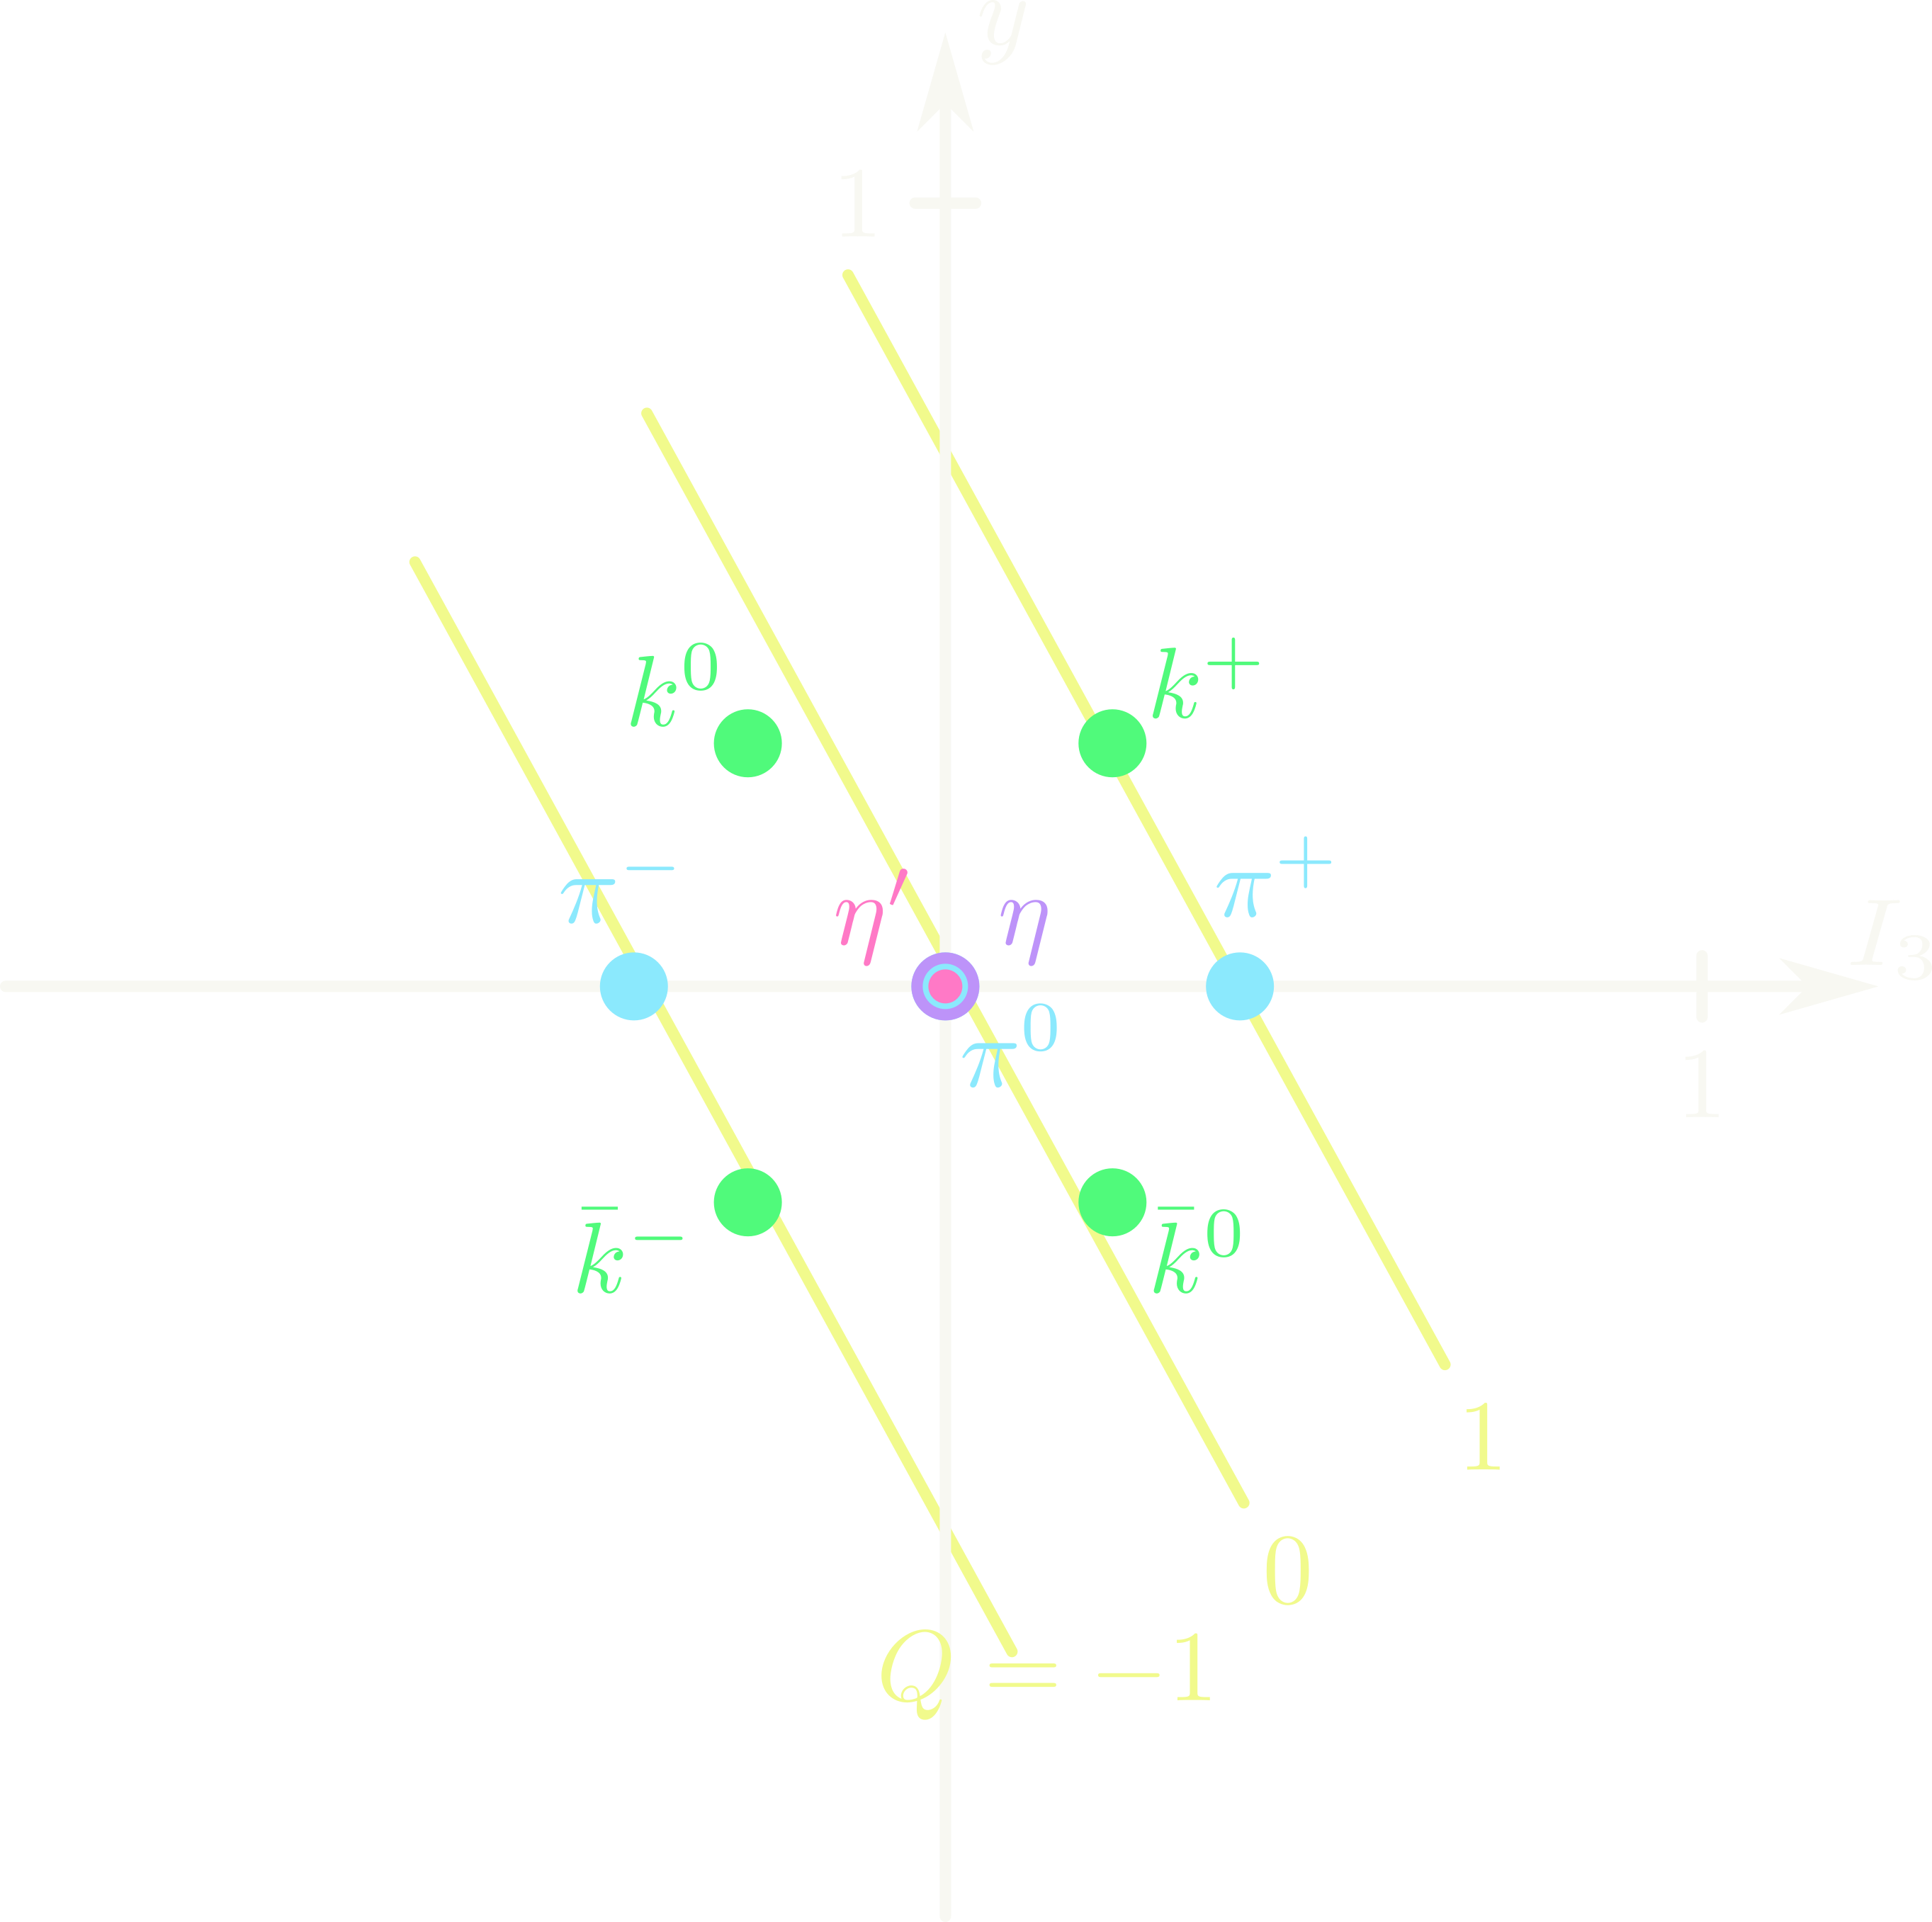
\includegraphics[width=0.5\textwidth]{mesons.png}
    \caption{The eightfold way}
    \label{fig:eightfold_way}
\end{figure}
Where $\eta$ is a $SU(2)$ singlet but a $SU(3)$ octet. and $\eta'$ is a $SU(3)$ singlet.

If $SU(3)_f$ was a good symmetry, expet all these 8 mesons to have similar mass. All of these obey
up to a factor of 2.

\paragraph*{Baryons} (222) or $3 \otimes 3 \otimes 3 = 10 \oplus 8 \oplus 8 \oplus 1$. The baryons
are antisymmetric as each quark is a fermion. Using the Young Tablauex
\begin{align*}
    3\otimes 3 = \begin{ytableau}
        a
    \end{ytableau} \otimes
    \begin{ytableau}
        b
    \end{ytableau}
    = 
    \begin{ytableau}
        3 & 4
    \end{ytableau}
    \oplus
    \begin{ytableau}
        3 \\
        2
    \end{ytableau}
    = \frac{3 \cdot 4}{1 \cdot 3} \oplus \frac{3 \cdot 2}{1 \cdot 2}
    = 6
\end{align*}
so
\begin{align*}
    6 \otimes 3 = 
    \begin{ytableau}
        a & b
    \end{ytableau}
    \otimes
    \begin{ytableau}
        c
    \end{ytableau}
    =
    \begin{ytableau}
        3 & 4 & 5
    \end{ytableau}
    \oplus
    \begin{ytableau}
        3 & 4 \\
        2
    \end{ytableau}
    =  \frac{3 \cdot 4 \cdot 5}{3 \cdot 2 \cdot 1} \oplus \frac{3 \cdot 4 \cdot 2}{1 \cdot 3 \cdot 1}
    = 10 \oplus 8
\end{align*}
This is a 10-plet as shown in the figure.
\begin{figure}[ht ]
    \centering
    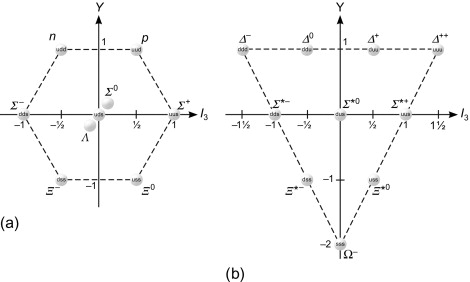
\includegraphics[width=0.5\textwidth]{baryons.png}
    \caption{The 10-plet of baryons}
    \label{fig:baryons}
\end{figure} 

\newpage
\subsection*{Lecture 7: \hfill  2/7/24}
\hrule \vspace{10px}

\paragraph*{Parity} (Discrete Symmetry) For a simple reflection on a $z$ axis
the point $A=(x, y, z)$ goes to $A' = (x, -y, z)$. But for parity operation we go to
$P(A) = (-x, -y, -z)$ or in the general form
\begin{align*}
    P(\vb{a}) = -\vb{a}
\end{align*}
also known as inversion. Taking the parity again we get
\begin{align*}
    P^2(\vb{a}) = P(-\vb{a}) = \vb{a}
\end{align*}
Thus it has a discrete $Z_2$ symmetry.

\paragraph*{Pseudo-vector} (axial vector) for a pseudo vector $\vb{c}$
\begin{align*}
    P(\vb{c}) = \vb{c}
\end{align*}
where cross products (of two vectors) are pseudo-vectors. For example
\begin{align*}
    \vb{c} = \vb{a} \cross \vb{b}
\end{align*}
and
\begin{align*}
    P(\vb{c}) = P(\vb{a} \cross \vb{b}) = (-\vb{a}) \cross (-\vb{b}) = \vb{c}
\end{align*}
e.g. of pseudo-vectors:
\begin{itemize}
    \item Torque: $\vb{\tau} = \vb{r} \cross \vb{F}$
    \item Angular momentum: $\vb{L} = \vb{r} \cross \vb{p}$
    \item Magnetic field: $\vb{B} = \vb{E} \cross \vb{v}$
\end{itemize}
But for the lorentz force 
\begin{align*}
    \vb{F} = q \qt(\vb{E} + \frac{1}{c} \vb{v} \cross \vb{B})
\end{align*}
the cross product of a vector and a pseudo-vector is a vector, so the lorentz force is a vector. 
Also from the general definition
\begin{align*}
    P(\vb{F}) = \frac{q}{c} P(\vb{v}) \cross P(\vb{B}) = \frac{q}{c} (-\vb{v}) \cross (-\vb{B}) = - \vb{F}
\end{align*}

The weak interaction violates parity\dots

\paragraph*{Scalar} For a scalar $s = \vb{a} \cdot \vb{b}$ is invariant under parity:
\begin{align*}
    P(s) = P(\vb{a} \cdot \vb{b}) = (-\vb{a}) \cdot (-\vb{b}) = \vb{a} \cdot \vb{b} = s
\end{align*} 
for a pseudo-scalar $p$ (a dot product of a vector and pseudo-vector):
\begin{align*}
    P(p) = P(\vb{a} \cdot (\vb{b} \cross \vb{c})) = P(\vb{a}) P(\vb{b} \cross \vb{c})
    = -\vb{a} (\vb{b} \cross \vb{c}) = -p
\end{align*}
So the partities of the four types of quantities:
\begin{itemize}
    \item Scalar: $P(s) = s$
    \item Pseudo-scalar: $P(p) = -p$
    \item Vector: $P(\vb{v}) = -\vb{v}$
    \item Pseudo-vector: $P(\vb{c}) = \vb{c}$
\end{itemize}

\paragraph*{Intrinsic Parity} The parity of a fermion is
\begin{align*}
    P(\text{fermion}) = - P(\text{anti-fermion})
\end{align*}
for bosons
\begin{align*}
    P(\text{boson}) = P(\text{anti-boson})
\end{align*}
For composite particles i.e. mesons $q\bar q$ and baryons $qqq$:
\begin{align*}
    P(\text{meson}) = -1 \qor (+1)(-1) = -1
\end{align*}
Since mesons are two pairs (particle, antiparticle) the parity is always negative. For baryons we 
can only have a positive parity:
\begin{align*}
    P(\text{baryon}) = (+1)^3 = +1
\end{align*}
For spherical harmonics $Y_l^m(\theta,\phi)$
under parity of each term:
\begin{align*}
    \vb{r} \to -\vb{r} \qquad \theta \to - \theta \qquad \phi \to \pi + \phi
\end{align*}
so
\begin{align*}
    P(Y_l^m(\theta, \phi)) = (-1)^l Y_l^m(\theta, \phi)
\end{align*}
and for excited states
\begin{align*}
    P = (-1)^l \times P(\text{ground state})
\end{align*}
where $l$ is the orbital angular momentum.

\paragraph*{Parity Violation} THe $\theta-\tau$ puzzle: given two particles
\begin{align*}
    \theta^+ \to \pi^+ + \pi^0 \qquad P = +1 \\
    \tau^+ \to \pi^+ + \pi^0 + \pi^0 \qquad P = -1
\end{align*}
the same two particles are found to be the same particle $K^+$ having the same mass and lifetime, 
but this violates the parity. To solve this puzzle came from the Colmbia University known as 
Wu's experiment \href{https://en.wikipedia.org/wiki/Wu_experiment}{(wikipedia)}:
\begin{align*}
    _{27}^{60} \text{Co} \to _{28}^{60} \text{Ni} + e^- + \bar \nu_e
\end{align*}
The Cobalt has a spin state of $J = 5$, the Nickel has spin $J = 4$ and the spin states of the 
electron-antielectron pair is $J = 1$. The electron is always emitted in the direction opposite of
the Cobalt spin, and when the magnetic field was inverted, the electrons were emitted in the
opposite direction of nuclear spin. This breaks parity, because in the mirror world, the spin of the
electron would be in the same direction as the nuclear spin.

\paragraph*{Helicity} From spin $\vb s$ and momentum $\vb p$ we can define the helicity
\begin{align*}
    \lambda = \frac{\vb{s} \cdot \vb{p}}{\abs{\vb{s}} \abs{\vb p}} \\
    =\begin{cases}
        +1 & \text{right-handed} \\
        -1 & \text{left-handed}
    \end{cases}
\end{align*}
But this depends on the reference frame. e.g. for a case where $\vb p$ is faster and in the same
direction of $\vb s$ the helicity is $\lambda = +1$, but in the reference frame faster that $\vb p$
the helicity is $\lambda = -1$.

\paragraph*{Massless Particles} For massless particles the helicity is the same in all reference
frames because the speed is always $c$ and thus the helicity is well-defined. For an electron, we
can get a frame where the momentum is different for changes in reference frames.

\paragraph*{Back to Wu's experiment} The spin of the electron and neutrino are in the same direction 
as the spin of the Cobalt and Ni. 

\paragraph*{Note:}In the SM 
\begin{itemize}
    \item neutrinos are always left-handed; $\lambda = -1$
    \item anti-neutrinos are always right-handed; $\lambda = +1$
\end{itemize}

Thus the electron momentum is in the opposite direction of spin as shown in Figure \ref{fig:helicity}

\begin{figure}[ht]
    \centering
    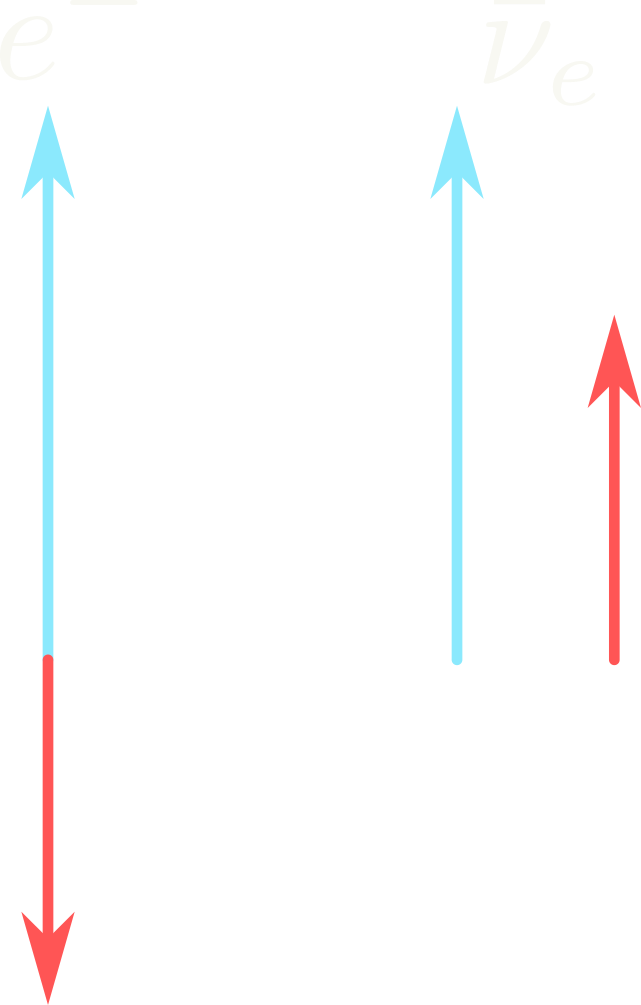
\includegraphics[width=0.2\linewidth]{helicity.png}
    \caption{Wu's experiment}
    \label{fig:helicity}
\end{figure}

\paragraph*{Another Example} Pions and muons
\begin{align*}
    \pi^+ \to \mu^+ + \nu_\mu \qor  \to e^+ + \nu_e
\end{align*}
From the comparison of masses
\begin{align*}
    m_\pi = \qty{140}{\MeV} \qquad m_\mu = \qty{105}{\MeV} \qquad m_e = \qty{0.511}{\MeV}
\end{align*}
we would think the small mass reaction would be more likely due to the higher velocity, but this
is not the case. For the pion the spin is 0, so the combination of spin will be in opposite directions.
From Figure \ref{fig:pion_eg} we can see that the anti-leption(anti particle) must be left-handed
and thus the lepton must also be left-handed. This is a parity violation.
\begin{figure}[ht]
    \centering
    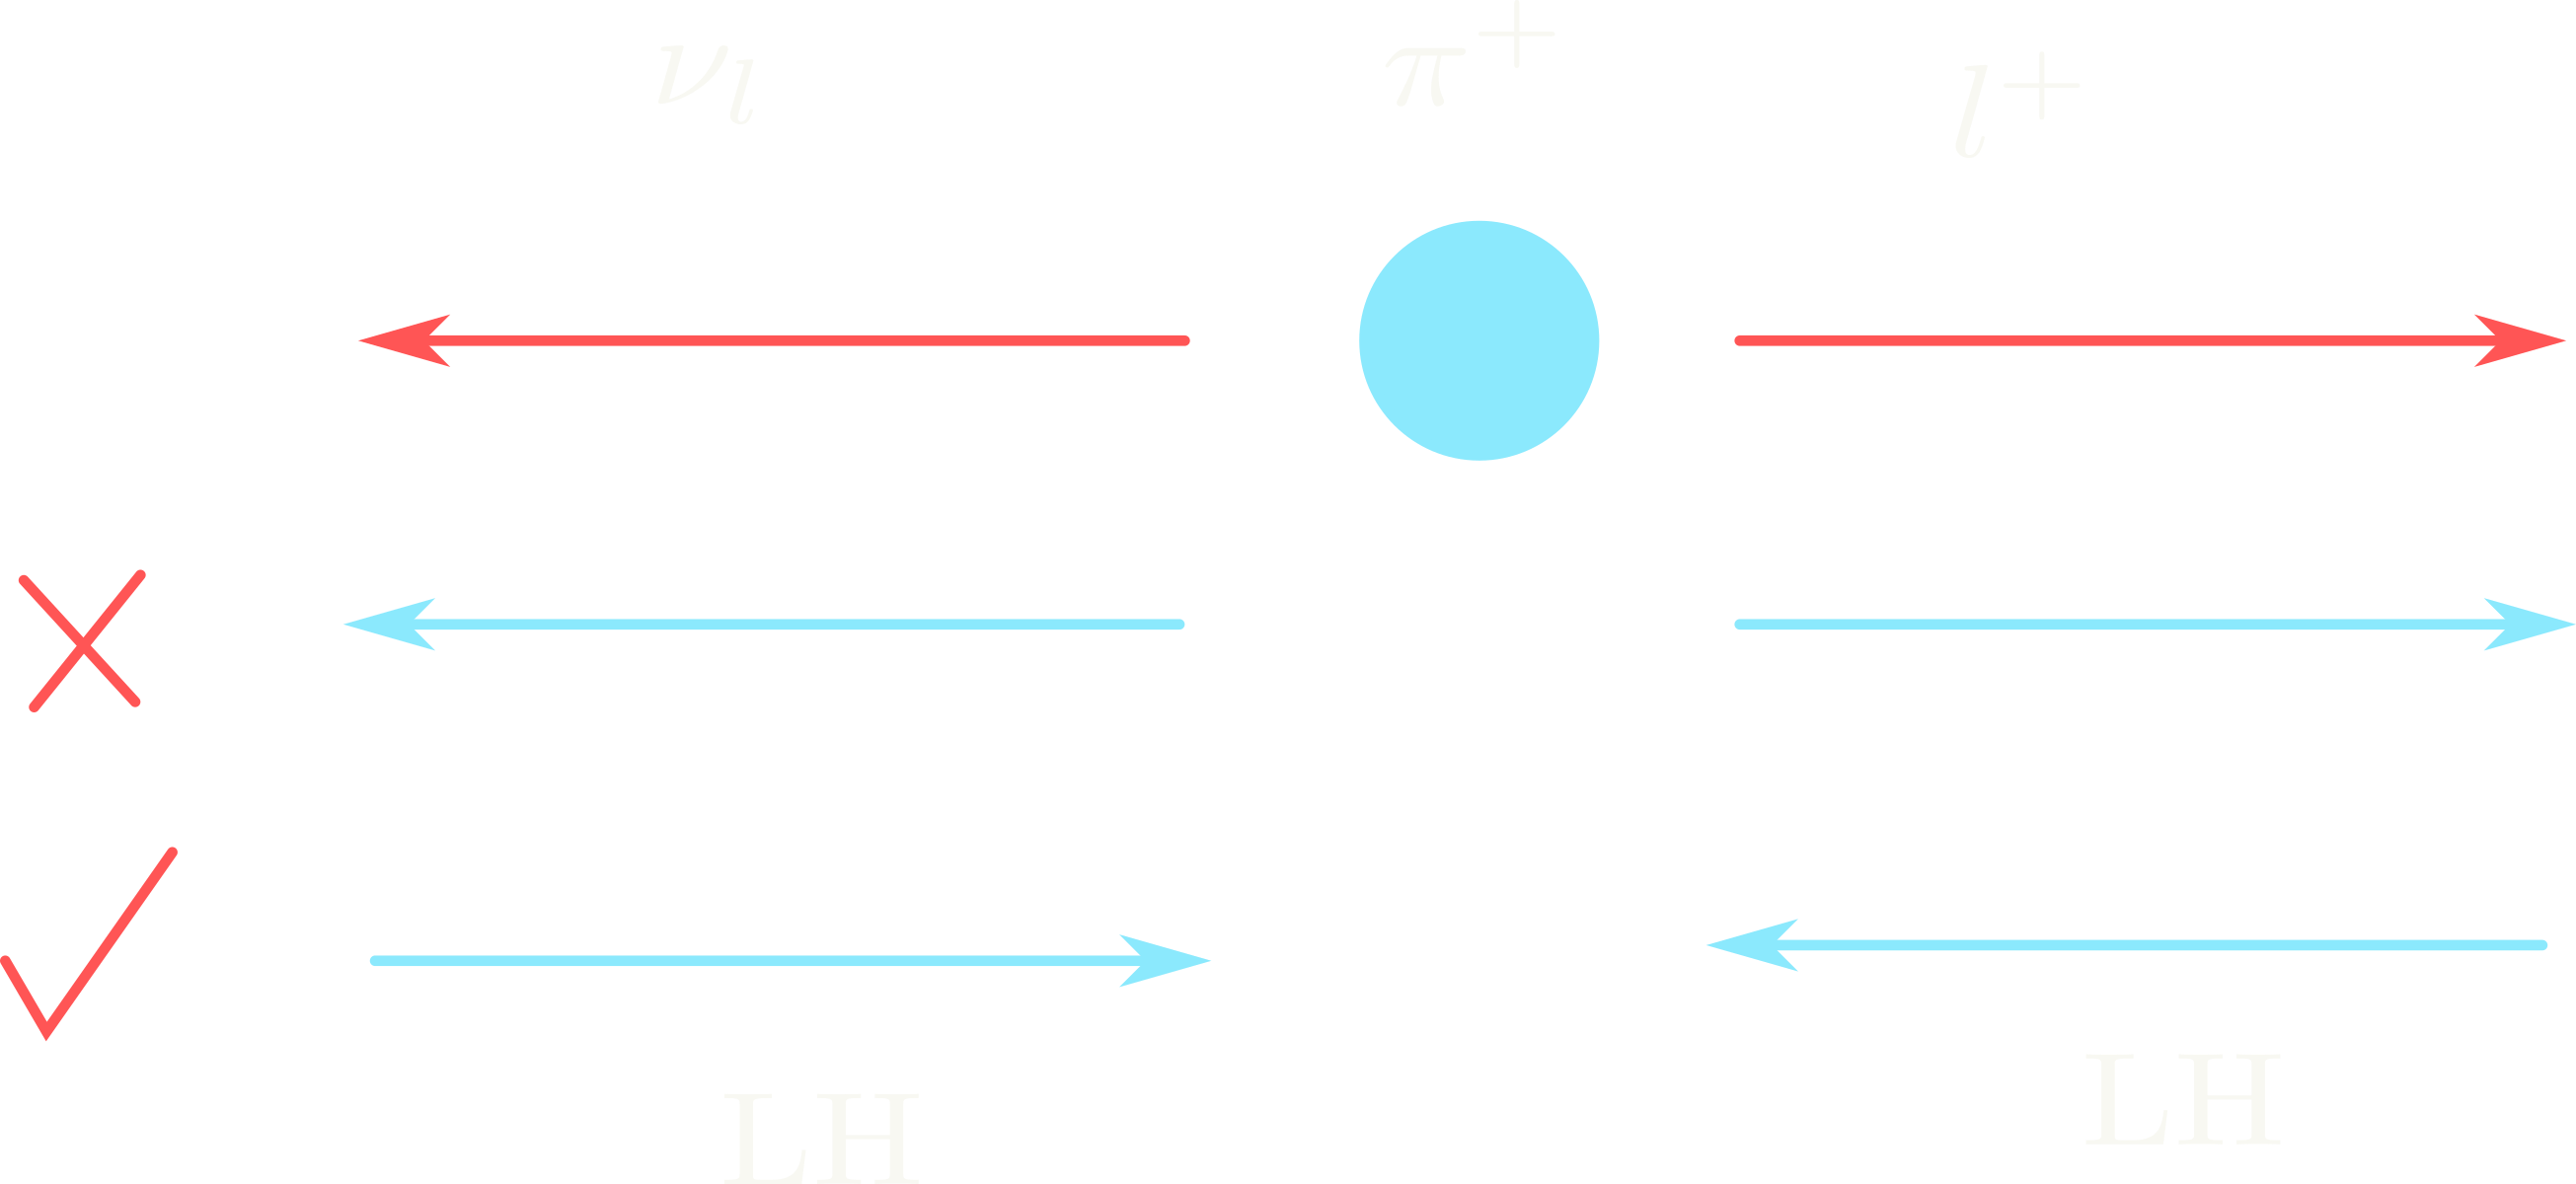
\includegraphics[width=0.5\textwidth]{pion_eg.png}
    \caption{Pion decay}
    \label{fig:pion_eg}
\end{figure}
Thus the less favored reaction $u^+ + \nu_\mu$ is seen 99.7\% of the time.
\paragraph*{} Anti-charged lepton has to be left-handed in this process of appoximate
\begin{align*}
    \Gamma \propto m_\ell^\beta
\end{align*}
where $\Gamma$ is the decay rate.

\paragraph*{Muon decay}
\begin{align*}
    \mu^- \to e^- + \bar \nu_e + \nu_\mu
\end{align*}
This 3 body decay for a polarized muon (choosing the handedness of the muon) we have the following
possiblities:
\begin{enumerate}
    \item LH
    \item RH
\end{enumerate}
For maximum energy to the electron, the electron goes in one direction while the neutrinos go in the
opposite direction as shown in Figure \ref{fig:muon_decay}. From this the RH case is less favored
than the LH case because of the helicity of the neutrinos.
\begin{figure}[ht]
    \centering
    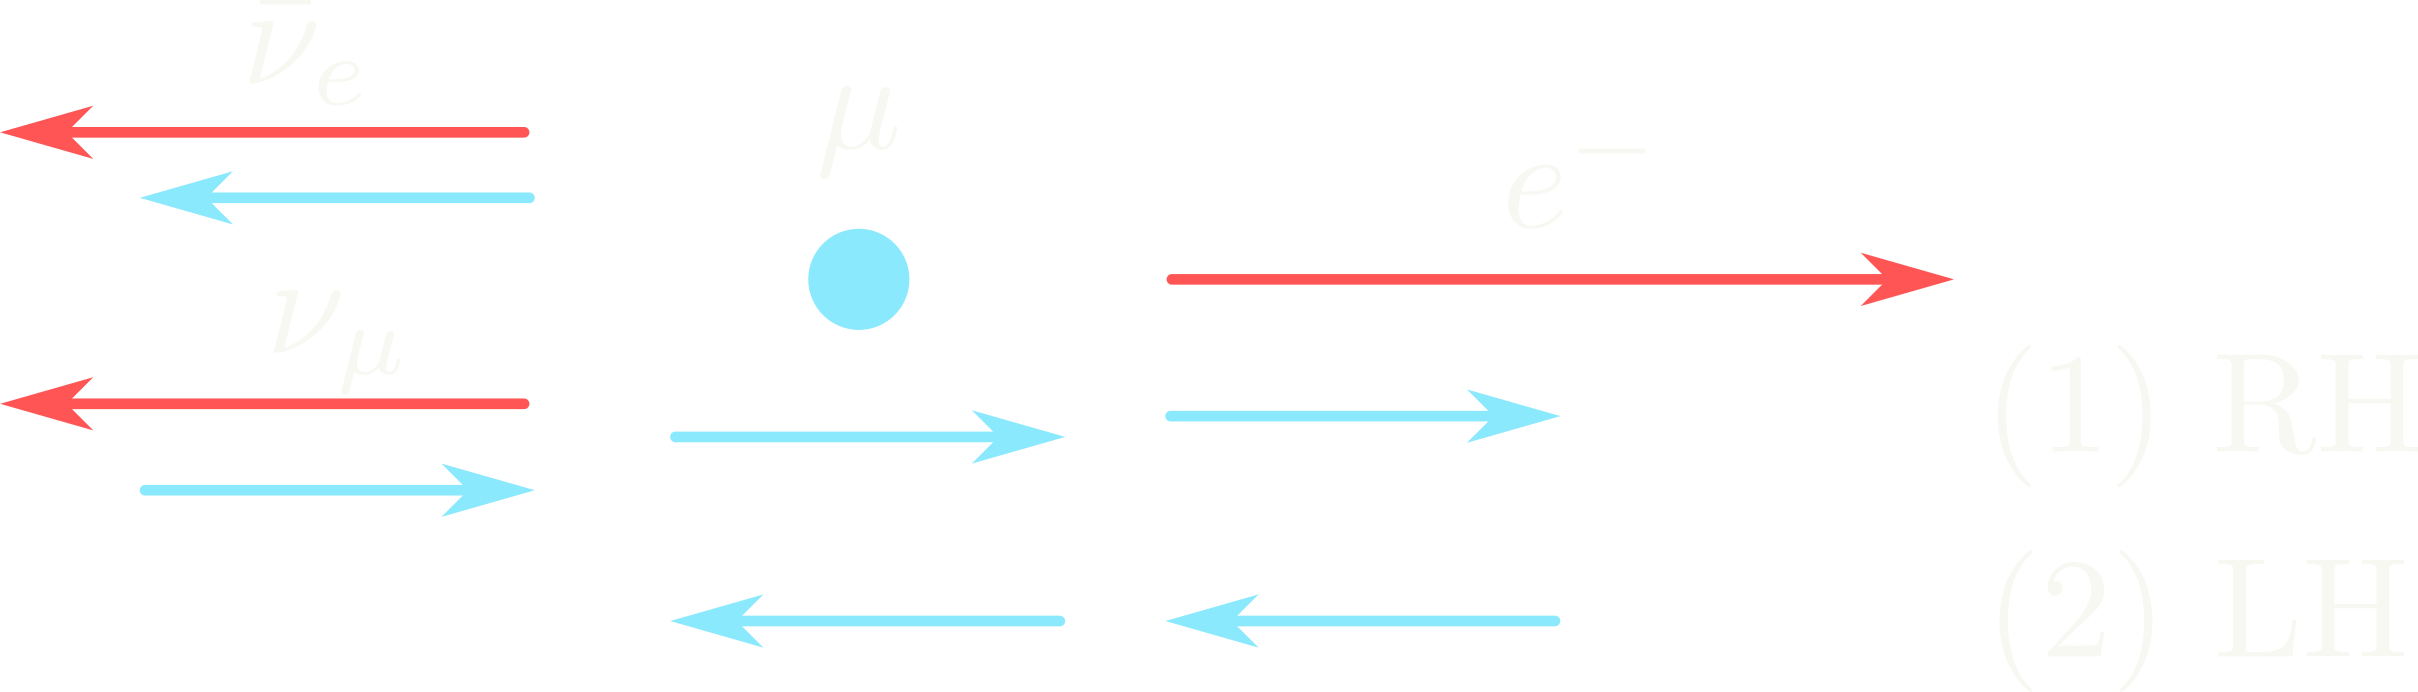
\includegraphics[width=0.5\textwidth]{muon_decay.png}
    \caption{Muon decay}
    \label{fig:muon_decay}
\end{figure}

\newpage
\subsection*{Lecture 8: \hfill  2/9/24}
\hrule \vspace{10px}

\paragraph*{Quiz Review}:
\begin{enumerate}
    \item The neutrino is an eigenstate of partity (neutrino has handedness)
    \begin{align*}
        P \ket{\nu}_L = \pm \ket{\nu}_L x \qquad A\ket \psi = \lambda \ket \psi
        \qquad P^2 = 1
    \end{align*}
    but $\ket \nu_R$ does not exists!
    \item Charge Conjugation ($C$)
    \begin{align*}
        C \ket m = \ket{\bar m}
    \end{align*}
    taking the charge conjugation twice
    \begin{align*}
        C^2 \ket m = C(C\ket m) = C\ket{\bar m} = \ket m \\
        \implies C^2 = 1 \implies C = \pm 1 \qqtext{$Z_z$-symmetry}
    \end{align*}
    So if $\ket m$ is an eigenstate of $C$ then
    \begin{align*}
        C \ket m = \pm \ket m = \ket{\bar m} \implies \ket m = \pm \ket{\bar m}
    \end{align*}
    e.g. For charged particles:
    \begin{align*}
        C \ket{\pi^+} = \ket{\pi^-}
    \end{align*}
    and for some neutral particles the charge conjugation is the same as the particle.
    One exception is the neutron
    \begin{align*}
        C\ket n = \ket{\bar n}
    \end{align*}
    and for the violation of Charge conjugation: the neutrino
    \begin{align*}
        C \ket \nu_L = \ket{\nu_L} \times
    \end{align*}
    here $C$ must be violated (in weak interactions) but preserved in strong \& EM interactions.
    \item G-parity: defined as
    \begin{align*}
        G = C R
    \end{align*}
    where $R$ is a rotation. From the 8-fold way, we can get from $\pi^+$ to $\pi^-$ by reflecting 
    it about the hypercharge axis or rotation by $2\pi$ in the $I_2$ axis and then taking its 
    charge conjugation:
    \begin{align*}
        G = C e^{i\pi I_2}
    \end{align*}
    so
    \begin{align*}
        G\ket{\pi^+} = C e^{i\pi I_2} \ket{\pi^+} = C \ket{\pi^-} = \ket{\pi^+}
    \end{align*}
    finding the G-parity of $K^+$: from the 8-fold way(Figure \ref{fig:eightfold_way}) we know that
    rotating $K^+$ actually gives us $K^0$ so
    \begin{align*}
        G \ket{K^+} = C e^{i\pi I_2} \ket{K^+} = C \ket{K^0} = \ket{\bar K^0}
    \end{align*}
    \paragraph*{Neutral Pion Decay} $\pi^0 \to \gamma + \gamma$ is a EM interaction (particle
    antiparticle pair: $(u\bar u - d \bar d)/\sqrt{2}$).
    \begin{align*}
        \pi^0 \to \gamma + \gamma
    \end{align*}
    The partity on the LHS is $P = -1$ and on the RHS $P = (-1)^2 = +1$. For the photon
    of spin:
    \begin{align*}
        S = 1, \qquad S_z = +1, \cancel{0}, -1 
    \end{align*}
    there is no longitudinal polarization $S_z = 0$, and the transverse polatization of the EM wave
    $S_z = \pm 1$ is the helicity. So the helicity of the photons must be the same; either
    $\lambda = \ket {++}$ or $\lambda = \ket{--}$. This is not an eigenstate of partity. The two 
    photons must have aligned polarizations. We also need to find $p$ in
    \begin{align*}
        \lambda = \frac{\vb{S} \cdot \vb{p}}{\abs{\vb{S}} \abs{\vb{p}}}
    \end{align*}
    where we know
    \begin{align*}
        p\ket + = \ket - \quad p\ket - = \ket + \quad p\ket{++} = \ket{--}
    \end{align*}
    we can write a linear combination of the two states
    \begin{align*}
        \ket{\psi_1} = \frac{1}{\sqrt{2}} \qt(\ket{++} + \ket{--}) \\
        \ket{\psi_2} = \frac{1}{\sqrt{2}} \qt(\ket{++} - \ket{--})
    \end{align*}
    for
    \begin{align*}
        P\ket{\psi_1} = \ket{\psi_1} \qqtext{(even parity)} \\
        P\ket{\psi_2} = -\ket{\psi_2} \qqtext{(odd parity)}
    \end{align*}
    This is similar to quantum optics where polarization is used:
    \begin{align*}
        \ket{+} = \frac{1}{\sqrt{2}} \qt(\ket{x} + i\ket{y}) \qquad
        \ket{-} = \frac{1}{\sqrt{2}} \qt(\ket x - i\ket y)
    \end{align*}
    we know the G parity is 
    \begin{align*}
        G = (-1)^I
    \end{align*}
    \item Pion decay to muon and neutrino: For the mesons
    \begin{align*}
        C = (-1)^{l+s}
    \end{align*}
    where we have two types: Pseudoscalars ($s = 0$) e.g $\pi, K$ with $C = (-1)^l$ and 
    vector mesons ($s = 1$) e.g. $\rho, K^*$ with $C = (-1)^{l+1}$. For $\rho$ we know that 
    $I(\rho) = 1$ from the 8-fold way, as well as $I(\eta) = 0$ so $\rho \to 3\pi$ and 
    $\eta \to 2\pi$ are allowed. 
    \paragraph*{CP} 
    \begin{align*}
        P\ket{\nu_L} = \ket{\nu_R} \times \\
        CP \ket{\nu_L} = C\ket{\nu_L} = \ket{\bar \nu_R}
    \end{align*} 
    where the P is violated due to the handedness of the neutrino, but the CP is conserved. applying
    CP on to the charged pion decay:
    \begin{align*}
        \pi^+ \to \mu^+ + \nu_\mu
    \end{align*}
\end{enumerate}
\subsection*{CP Violation}
For an oscillation of a neutral kaon $K^0(d\bar s$) and $\bar K^0 (\bar d s)$. Because K's are 
pseudoscalars:
\begin{align*}
    P\ket{K^0} = -\ket{\bar K^0} \qquad P\ket{\bar K^0} = \ket{\bar K^0}
\end{align*}
and the charge conjugation is
\begin{align*}
    C\ket{K^0} = \ket{\bar K^0} \qquad C\ket{\bar K^0} = \ket{K^0}
\end{align*}
and the CP is
\begin{align*}
    CP\ket{K^0} = -\ket{\bar K^0} \qquad CP\ket{\bar K^0} = -\ket{K^0}
\end{align*}
which are not eigenstates of CP, so taking a linear combination of the two states
\begin{align*}
    \ket{K_1} = \frac{1}{\sqrt{2}} \qt(\ket{K^0} - \ket{\bar K^0}) \qquad
    \ket{K_2} = \frac{1}{\sqrt{2}} \qt(\ket{K^0} + \ket{\bar K^0})
\end{align*}
the CP of the two states are
\begin{align*}
    CP\ket{K_1} = \ket{K_1} \qquad CP\ket{K_2} = -\ket{K_2}
\end{align*}
which are eigenstates of CP. Karons decay to pions(lightest meson): to either 2 or 3 pions. From the
phase space, the 2 pion decay is more likely than the 3 pion decay because faster particles are
more likely to decay: A kaon with 490 MeV to 2$\times$140 = 280 MeV is more likely than 3$\times$140
= 420 MeV. The 2 pion decay has CP
\begin{align*}
    CP\ket{\pi^+\pi^-} = (-1)^2 \ket{\pi^+\pi^-} = \ket{\pi^+ \pi^-} \\
    CP\ket{\pi^+\pi^-\pi^0} =  (-1)^3 \ket{\pi^+\pi^-\pi^0} = -\ket{\pi^+\pi^-\pi^0}
\end{align*}
so the 2 pion decay is CP even and the 3 pion decay is CP odd. If CP were conserved,
\begin{align*}
    \ket{K_1} \to \ket{2\pi} \qquad \ket{K_2} \to \ket{3\pi}
\end{align*}
so we call this fast decay $K_S$ meaning short ($\num{9e-11}{sec}$) and the slow decay $K_L$ meaning
long ($\num{5e-8}{sec}$) or
\begin{align*}
    \ket{K_1} \equiv \ket{K_S^0} \qquad \ket{K_2} \equiv \ket{K_L^0}
\end{align*}
from a nobel prize winning experiment, a detector far away would be expected to see mostly $K_L$ but
the experiment showed that we saw some amount to the 2 pion decay:
\begin{align*}
    \ket{K_L^0} = \frac{1}{\sqrt{1 + \epsilon^2}} \qt(\ket{K_S^0} + \epsilon \ket{K_L^0})
\end{align*}
where $\epsilon = \num{2.3e-3}$ characterizes CP violation.
\end{document}